\begin{center}
    \section*{CAPÍTULO I}
    \addcontentsline{toc}{section}{RESEÑA HISTÓRICA}
    \vspace*{0.5in}
    \textbf{RESEÑA HISTÓRICA}
\end{center}

Su filosofía es desarrollar talentos y compartir 
conocimientos con las nuevas generaciones, 
con el objetivo de Impulsar el desarrollo de empresas y comunidades a nivel mundial, implementando 
tendencias tecnológicas y nuevos modelos de negocio, para posicionar y mantener a sus clientes con éxito en el 
mercado actual y futuro.\\
 
Fue fundada en 2017 por el Lic. Luis Sandoval 
y Ing. Luis Güette  reclutando a jóvenes venezolanos 
de diferentes universidades en la cual participaron mas de 
1000 estudiantes.\\

En sus inicios realizaron mas de 50 propuestas a nivel 
nacional e internacional para diversos clientes basados 
en la estandarización de procesos internos, desarrollo web 
y automatización.\\

Actualmente se han expandido a áreas como: Blockchain, IOT, 
VR/AR, Inteligencia artificial, Diseño de Productos y 
Finanzas.\\

Sus proyectos mas destacados han sido: diseño de SCADA 
para sistemas fotovoltaicos, diseño SCADA para un sistema 
de energía eléctrica. Diseño de identidad corporativa, 
Diseño de maquina secadora de cemento,Diseño de maquina de 
concreto.\\

Actualmente Type trabaja desde Venezuela, México y Estados 
Unidos. se encuentra desarrollando plataformas web, 
aplicaciones para internet de las cosas y migración de datos a la nube. 
\\                      

\begin{center}
    \textbf{ORGANIGRAMA DE TYPE}
\end{center}

\begin{figure}[H]
    \centering
        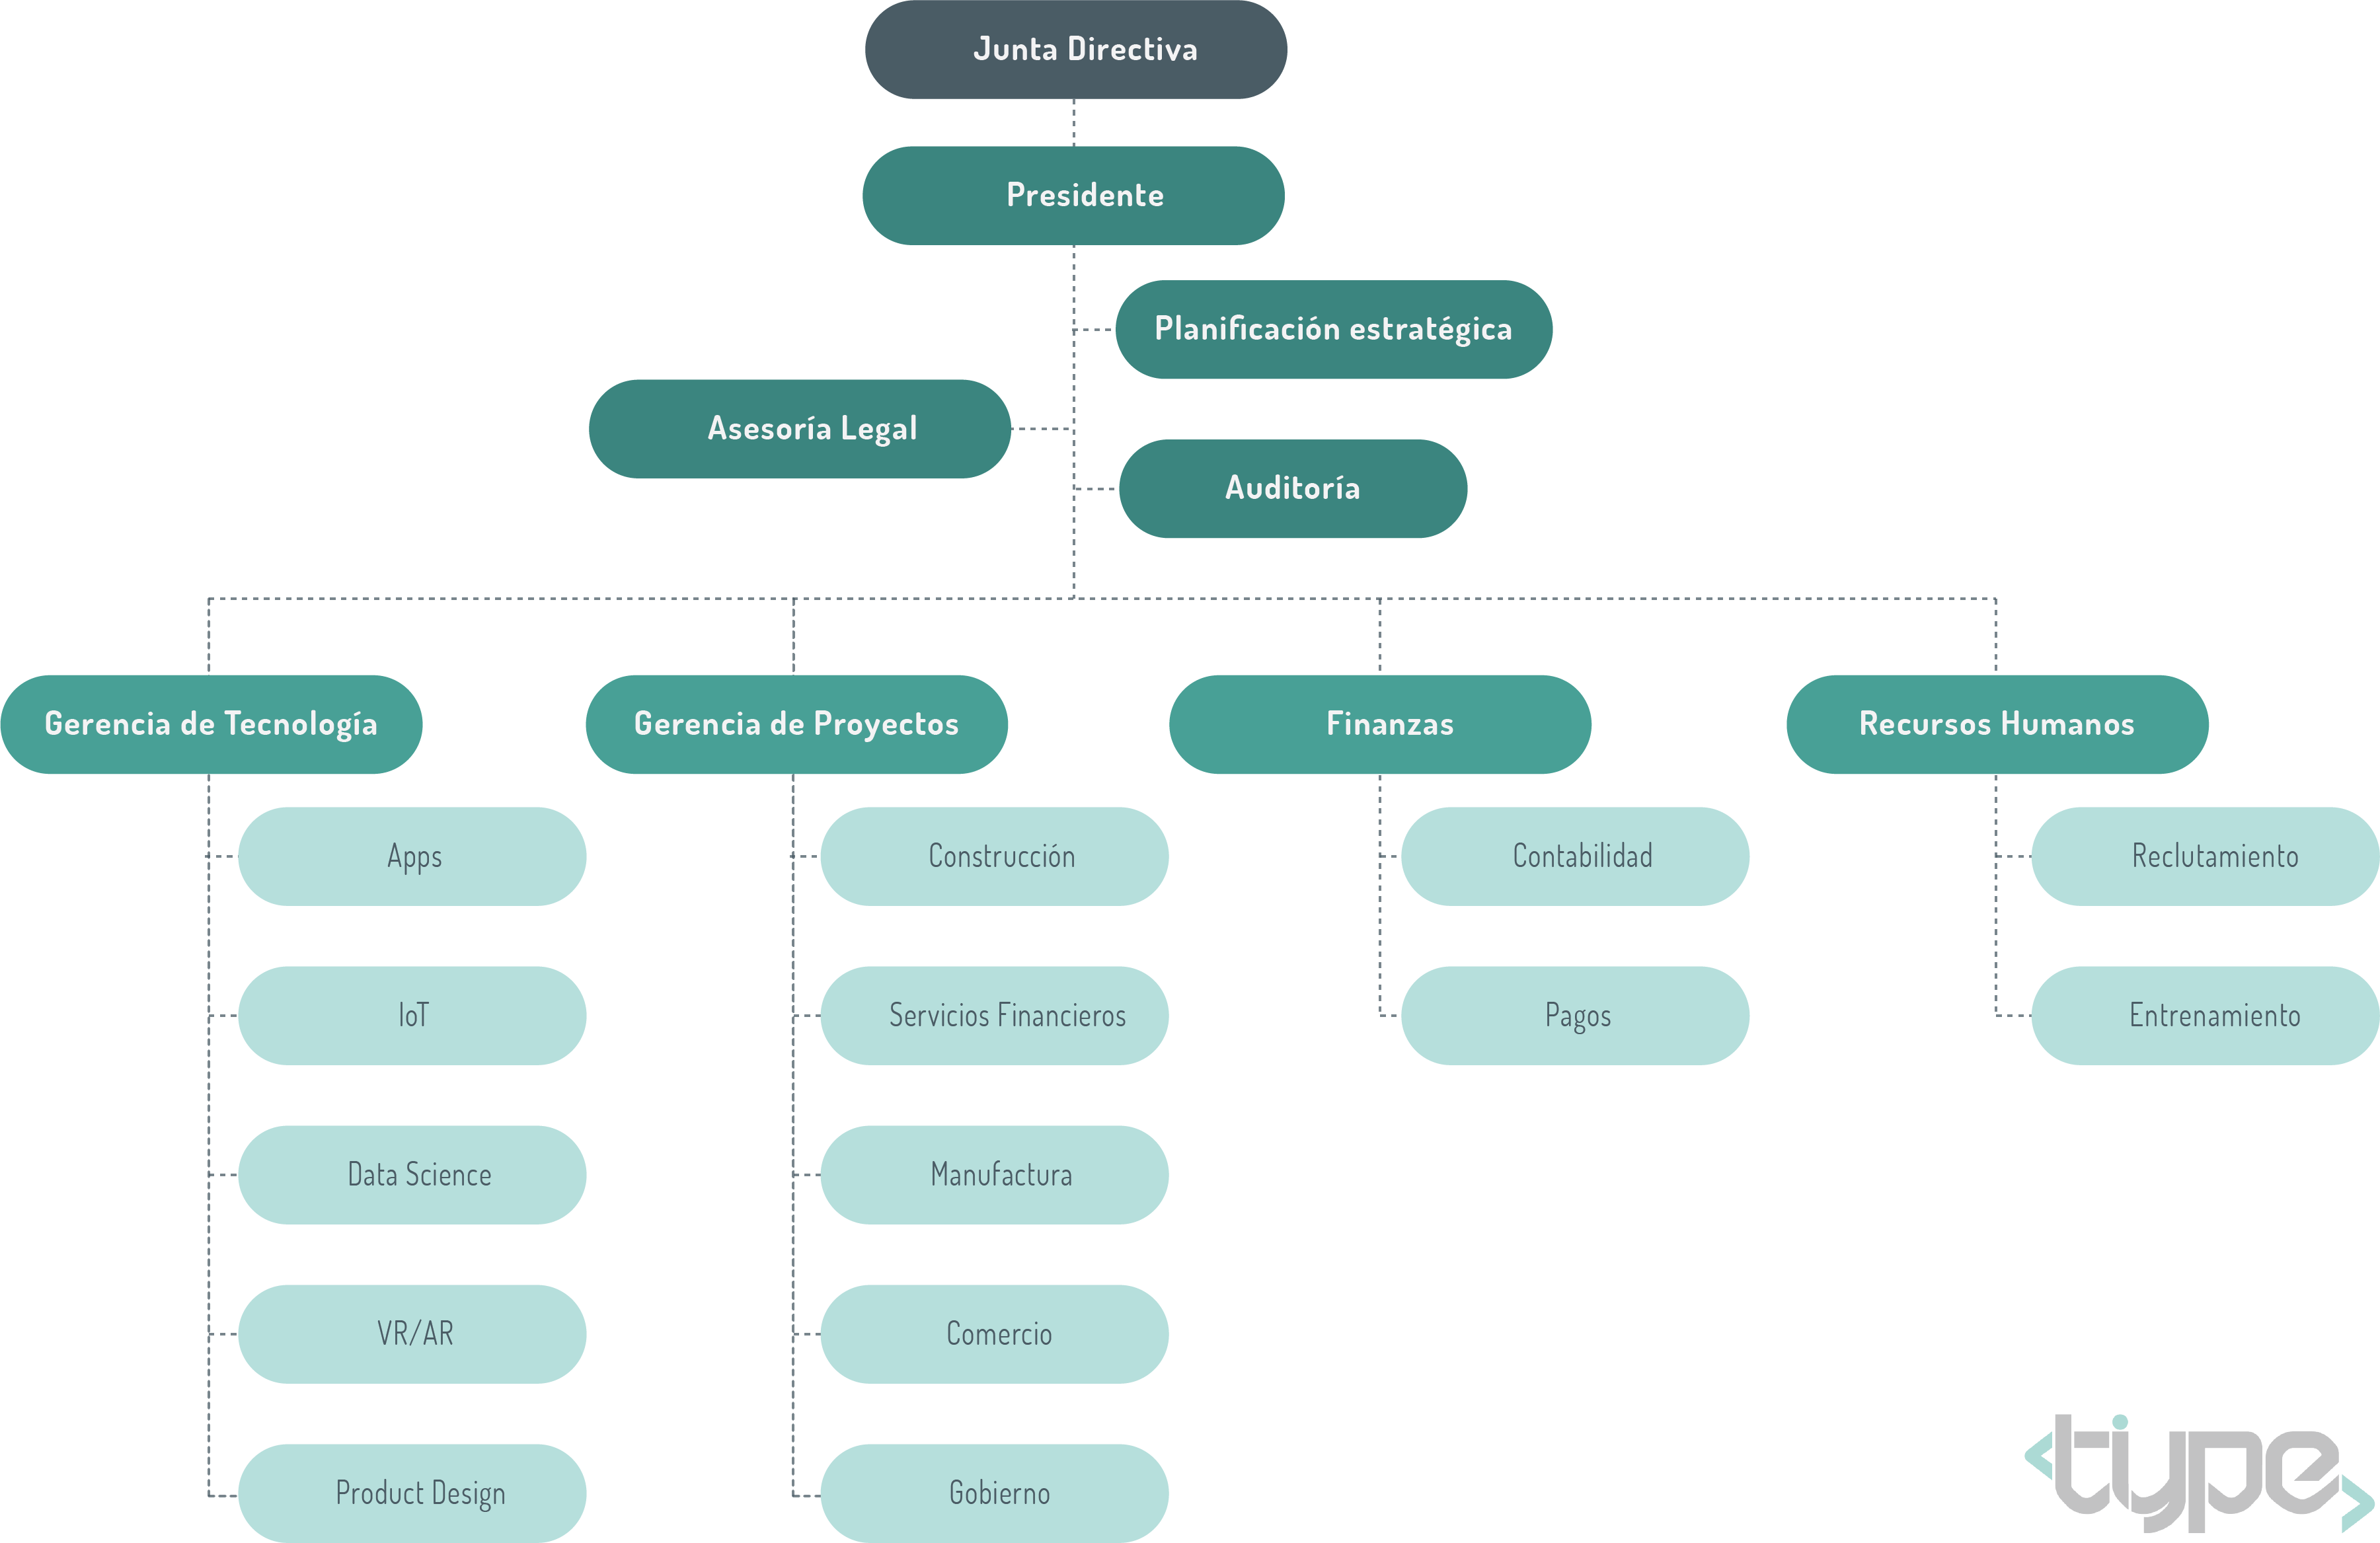
\includegraphics[scale=0.5]
        {Organigrama_type_07082019.png}
    \caption{Estructura de la empresa}
    \label{fig:my_label}
\end{figure}

\newpage